\documentclass[12pt,a4paper]{article}
\usepackage{geometry}
\geometry{left=2.5cm,right=2.5cm,top=2.0cm,bottom=2.5cm}
\usepackage[english]{babel}
\usepackage{amsmath,amsthm}
\usepackage{amsfonts}
\usepackage[longend,ruled,linesnumbered]{algorithm2e}
\usepackage{fancyhdr}
\usepackage{ctex}
\usepackage{array}
\usepackage{listings}
\usepackage{color}
\usepackage{graphicx}
\usepackage[hidelinks]{hyperref}
% \usepackage[colorlinks=true, linkcolor=blue, urlcolor=blue]{hyperref}  % 自訂連結顏色並移除方框
% Add the following lines
\usepackage{fontspec}
\usepackage[UTF8]{ctex}

\setmainfont{Sarasa Gothic TC}
\setCJKmainfont{Sarasa Gothic TC}
\setCJKsansfont{Sarasa Gothic TC}
\setCJKmonofont{Sarasa Gothic TC}
\begin{document}


\title{
  {
    \heiti Computer Graphics 第 4 次 Homework
  }
}


\date{
  \begin{tabular}{ll}
  2025/01/09 (生日前一天) & \hfill 
\includegraphics[width=0.06\textwidth]{img/cake.png} \\
  \end{tabular}
  }
\author{
  年級:{資工三}~~~~~~
  學號:{S11159005}~~~~~~
  姓名:{黃毓峰}~~~~~~
}


\maketitle
\newlength{\question}
\settowidth{\question}{XX}

\section*{{問題描述}}
繪製 3D 四面體(Tetrahedron),並在不同的體積分割次數(Depth)下計算並顯示其頂點數據。
為了更方便地調整分割層數,並加入物體自動旋轉控制,攝影機的操作
以及加入兩個光源,讓物件的繪製受到光源影響(shading),程式供右鍵選單可以調整。

\section*{實作/程式說明}

\noindent 新增主要功能包含:

\begin{itemize}
  \item 雙光源設定
  \item 法向量計算
\end{itemize}

\subsection*{核心演算法解說}

\begin{enumerate}
  \item \textbf{雙光源設定}:
    \begin{itemize}
        \item 使用 glEnable(GL\_LIGHTING) 啟用光照。
        \item 使用 glEnable(GL\_COLOR\_MATERIAL) 和 glColorMaterial(GL\_FRONT, GL\_AMBIENT\_AND\_DIFFUSE) 讓物體的顏色影響其漫射和環境光照。
        \item 使用 glLightfv` 設定每個光源的環境光、漫射光、鏡面反射光。
        \item 使用 glLightfv` 設定每個光源的位置。
        \item 使用 glEnable(GL\_LIGHT0) 和 glEnable(GL\_LIGHT1) 來啟用光源。
        \item 使用 glDisable(GL\_LIGHT0) 和 glDisable(GL\_LIGHT1) 來關閉光源。
    \end{itemize}
    
    實作如下 (有省略部份程式):
\begin{lstlisting}[language=C++,breaklines=true]
void init() {
    // ...
    glEnable(GL_LIGHTING);
    glEnable(GL_COLOR_MATERIAL);
    glColorMaterial(GL_FRONT, GL_AMBIENT_AND_DIFFUSE);

    GLfloat light_ambient[]   = {0.1f, 0.1f, 0.1f, 1.0f}; 
    GLfloat light_diffuse[]   = {1.0f, 1.0f, 1.0f, 1.0f};
    GLfloat slight_specular[] = {1.0f, 1.0f, 1.0f, 1.0f};

    glLightfv(GL_LIGHT0, GL_AMBIENT,   light_ambient);
    glLightfv(GL_LIGHT0, GL_DIFFUSE,   light_diffuse);
    glLightfv(GL_LIGHT0, GL_SPECULAR, slight_specular);
    // set light 1 as light 0
}

void display() {
    // ...
    if (light0_status) glEnable(GL_LIGHT0);
    else glDisable(GL_LIGHT0);

    if (light1_status) glEnable(GL_LIGHT1);
    else glDisable(GL_LIGHT1);

    GLfloat light0_position[] = {-0.0f, 0.0f, 0.65f, 0.0f};
    glLightfv(GL_LIGHT0, GL_POSITION, light0_position);
    GLfloat light1_position[] = {-0.3f, -0.25f, -0.5f, 0.0f};
    glLightfv(GL_LIGHT1, GL_POSITION, light1_position);
    // ...
}
\end{lstlisting}
\newpage
\item \textbf{法向量計算}:
    \begin{itemize}
      \item 法向量為垂直於表面的向量,用來計算光照。
      \item 計算方式為透過兩個邊向量的乘積來計算,並進行正規化。
    \end{itemize}
    \begin{lstlisting}[language=C++,breaklines=true]
void draw_triangle_with_normal(GLfloat p1[], GLfloat p2[], GLfloat p3[]) {
    GLfloat u[3], v[3], normal[3];
    for (int i = 0; i < 3; ++i) {
        u[i] = p2[i] - p1[i];
        v[i] = p3[i] - p1[i];
    }

    normal[0] = u[1]*v[2] - u[2]*v[1];
    normal[1] = u[2]*v[0] - u[0]*v[2];
    normal[2] = u[0]*v[1] - u[1]*v[0];

    GLfloat length = sqrt(normal[0]*normal[0] + normal[1]*normal[1] + normal[2]*normal[2]);
    for (int i = 0; i < 3; ++i) normal[i] /= length;

    glNormal3fv(normal);

    glBegin(GL_TRIANGLES);
    glVertex3fv(p1);
    glVertex3fv(p2);
    glVertex3fv(p3);
    glEnd();
}
\end{lstlisting}
  


\end{enumerate}
\newpage
\subsection*{程式架構}
\noindent 主要函數說明:
\begin{itemize}
\item \texttt{tetrahedron}:遞迴實現四面體細分
\item \texttt{draw\_triangle\_3d}:繪製四面體的四個面
\item \texttt{midpoint}:計算兩點的中點
\item \texttt{mouseButton}:處理滑鼠按鍵事件
\item \texttt{mouseMotion}:處理滑鼠移動事件
\item \texttt{idle}:用於動畫效果,定期更新旋轉角度
\item \texttt{display}:繪製場景,包含模型與攝影機設定
\item \texttt{processAxisMenu}:處理選單中選擇旋轉軸的事件
\item \texttt{processDirectionMenu}:處理選單中選擇旋轉方向的事件
\item \texttt{createMenu}:建立互動選單
\item \texttt{draw\_triangle\_with\_normal}:繪製四面體的四個面以及計算法向量
\end{itemize}

\section*{程式編譯環境}
\subsection*{電腦軟體系統簡介}
\begin{itemize}
  \item MacOS 15.2 - Darwin Kernel Version 24.2.0 - ARM64
  \item Apple clang version 16.0.0
  \item cmake version 3.31.3
  \item OpenGL - 4.1
\end{itemize}



\subsection*{GLFW函式庫名稱與版本}

\begin{itemize}
  \item freeglut - 3.6.0-2 
\end{itemize}
\newpage
\section*{編譯後的執行成果}
\begin{figure}[h]
  \centering
  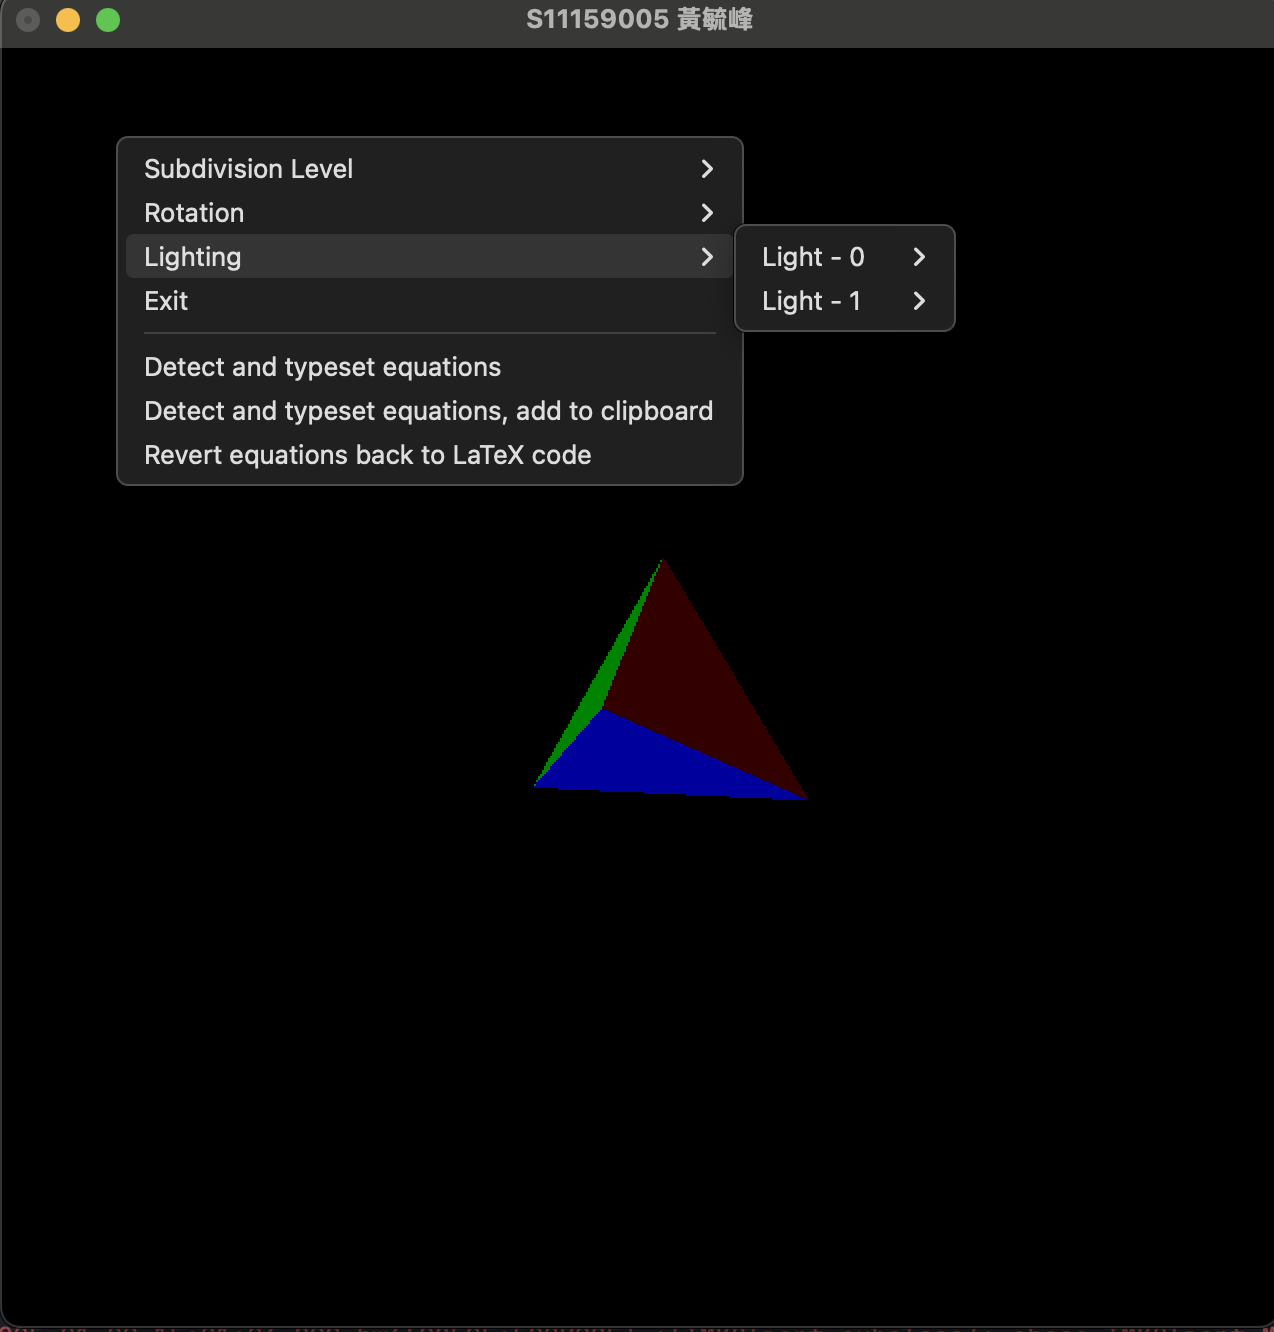
\includegraphics[width=0.8\textwidth]{img/hw4_result.png}
  \caption{執行結果}
\end{figure}

\section*{心得}
在這次的作業中,我學到MacOS 是一個很詭異的OS,對我又變開發環境了這次改用MacOS,讓我學會如何配置MacOS OpenGL環境,還有複習了我的數學以及學到更多圖學知識。

\section*{SourceCode}
\sloppy
\noindent \url{https://github.com/IDK-Silver/NUTN-CSIE-Code/tree/main/ComputerGraphics/hw4}




\end{document}
